\documentclass[a4paper,twoside]{article}

\usepackage{epsfig}
\usepackage{subcaption}
\usepackage{calc}
\usepackage{amssymb}
\usepackage{amstext}
\usepackage{amsmath}
\usepackage{amsthm}
\usepackage{multicol}
\usepackage{pslatex}
\usepackage{apalike}
\usepackage{algorithm2e}
\usepackage[bottom]{footmisc}
%% Additional packages required by this paper, loaded before SCITEPRESS.sty.
\usepackage{graphicx}
\usepackage{textcomp}
\usepackage{xcolor}
\usepackage{booktabs}
\usepackage{multirow}
\usepackage{url}
\usepackage{tikz}
\usetikzlibrary{arrows.meta, positioning, shapes, backgrounds}
\usepackage{SCITEPRESS}     % Please add other packages that you may need BEFORE the SCITEPRESS.sty package.

\begin{document}

\title{VLM Substitution in Autonomous Driving Data: Per-Class Behavioral Shifts in Scene Annotation}

\author{\authorname{Toomas Tahves\sup{1}\orcidAuthor{0009-0008-0050-2146}, Mauro Bellone\sup{2,3}\orcidAuthor{0000-0003-3692-0688} and Raivo Sell\sup{1}\orcidAuthor{0000-0003-1409-0206}} \affiliation{\sup{1}Department of Mechanical and Industrial Engineering, Tallinn University of Technology, Estonia} \affiliation{\sup{2}FinEst Centre for Smart Cities, Tallinn University of Technology, Estonia} \affiliation{\sup{3}Department of Computer Science and Engineering, Universitas Mercatorum, Rome, Italy} \email{\{toomas.tahves, mauro.bellone, raivo.sell\}@taltech.ee} }

\keywords{Multi-Agent Systems, Vision-Language Models, Prompt Engineering, Annotation Pipelines, Semantic Segmentation, Autonomous Driving.}

\abstract{
Vision–language models (VLMs) are now used as multi‑agent judges in large annotation pipelines, where each agent operates under a fixed role, a fixed prompt, and a small output vocabulary.
When VLM backend models are replaced, then there is no established way to measure where model behaviour changes inside a deployed system.
We introduce a controlled, per‑agent, per‑class process for backend substitution and apply it to a SAM‑based mask‑verification pipeline on the Zenseact Open Dataset.
Two open‑weight VLMs, LLaVA‑1.6‑34B and Qwen2.5‑VL‑72B, are run over the same 4{,}110 driving frames and 90{,}176 mask proposals using identical prompts and identical non‑VLM inputs.
All comparisons are paired at mask level, the triage rule is recomputed once for both runs.
The two backends agree on only 57.0\% of the judgements about what object the cropped region contains, and the differences are strongly class‑dependent.
Relative to LLaVA, Qwen rejects far fewer signs and cyclists, yet rejects more vehicles and pedestrians, shifting which classes lose labels rather than the overall rejection rate.
In the final annotations, 18.8\% of masks (7.5 million pixels) are retained by one backend and removed by the other.
The largest divergence appears in the step that recovers objects missed by SAM, where the confirmation rate for human candidates drops from 85.9\% to 45.3\% when the backend is changed.
Reliable deployment therefore requires systematic per‑agent and per‑class validation on identical inputs.
}


\onecolumn \maketitle \normalsize \setcounter{footnote}{0} \vfill

\section{\uppercase{Introduction}}
\label{sec:introduction}

Delegating judgement to a language model has become a standard part of modern data pipelines.
The LLM-as-judge pattern~\cite{zheng2023judging} gives a model a narrow evaluative role, limits its output to a small vocabulary, and treats its verdict as one signal among several.
Vision–language models extend this idea to image data~\cite{liu2024llava,wang2024qwen2vl}, which makes them appealing for annotation auditing: a mask proposal, a crop, a fixed question, and a categorical answer.

Pipelines built this way inherit an engineering assumption that is rarely checked.
Because each agent is defined by a role and a prompt rather than by learned weights, the backend looks like a swappable component.
A practitioner who has validated a pipeline on one open model often expects to switch to a larger or cheaper one by changing a configuration entry.
Prompt tuning per model is not realistic at annotation scale.
That different models behave differently is obvious.
What is missing is a way to measure how differently and where, inside a working pipeline and on a dataset large enough for the answer to matter.
Substitution is usually reported as a single acceptance or confirmation rate per model, which cannot show which agent changed, which classes moved, or whether a shift came from the model or from a serving failure.

We build this measurement into a system where backend substitution can be isolated cleanly.
Three agents act on every SAM~\cite{kirillov2023sam} mask: a geometric consistency check, a segmentation‑quality model, and a crop‑level object‑identity judge.
A fourth agent recovers objects that SAM misses by issuing class‑specific prompts on regions where the segmentation model and SAM diverge; it is the only one that acts on the frame rather than on a proposed mask.
Only the two VLM‑based agents change when the backend changes; the consistency check and the segmentation‑quality model are computed once and shared across both runs.
Running two open‑weight VLM backends over the same 4{,}110 frames produces two annotation sets whose differences can be attributed directly to the VLM, because all non‑VLM inputs are held fixed and verified before comparison.

Our contributions are as follows.
We design an annotation system in which backend substitution can be isolated cleanly: agent roles, prompts, output vocabularies, and fallback behaviour are specified tightly enough that any change in outcomes can be attributed to the VLM rather than to the surrounding pipeline.
We introduce a controlled substitution process that measures portability per agent and per class, using paired mask-level comparisons over 90{,}176 mask proposals and 55{,}256 recovery candidates with all non-VLM signals held fixed.
We show that fixed prompts do not transfer uniformly: the two backends diverge sharply on small and human classes, and the overall acceptance rate hides a 41-point drop in cyclist and pedestrian confirmations.
Finally, we quantify the operational cost of the larger backend and relate that cost to the annotation distribution it produces.


\section{\uppercase{Related Work}}

Language models have increasingly been used as delegated judges in data pipelines.  
The LLM-as-judge pattern~\cite{zheng2023judging,wu2023llmjudge} shows that a model can evaluate another system’s output when given a structured prompt and a constrained response format, and this idea has already been applied to data annotation~\cite{gilardi2023chatgptannotator,li2023llmannotator,li2023llmdata}.  
Agent frameworks extend this approach by combining several such roles into pipelines with explicit delegation~\cite{xi2023agents,schick2023toolformer,wang2023voyager}, an idea that also appears in embodied decision-making~\cite{ahn2022saycan,huang2023inner,brohan2023rt2}.  
Most of this work evaluates the composed system as a whole and assumes that a role specification can be transferred across different models without changing behaviour.

That assumption is weakly supported.  
Prompt phrasing and format are known to shift model behaviour, and work on instruction form~\cite{wei2022chain} shows that even small changes in wording can alter what a model does.  
What is missing is a controlled substitution study at deployment scale, where two backends are run with identical prompts and identical non-model inputs, and the comparison is resolved per agent and per class rather than through a single aggregate rate.  
Research on foundation-model capability surfaces~\cite{bommasani2021opportunities} suggests that substitution is not neutral, but does not measure where these differences appear inside a working system.

Annotation auditing over SAM proposals introduces its own challenges.  
SAM~\cite{kirillov2023sam} produces class-agnostic masks without per-class prompts, which makes large-scale pseudo-annotation feasible but leaves semantic correctness unchecked.  
Filtering on confidence or cross-modal geometry~\cite{zou2019confidence,jaritz2020xmuda} cannot detect a plausible mask that carries the wrong class, which motivates the use of a semantic judge.  
Ensemble-style label-noise methods~\cite{malach2017decoupling,han2018co} further motivate requiring agreement before acting on a rejection.  
Our system combines these ideas, and this paper examines what happens when the semantic judge itself is replaced.

\begin{figure}[t]
    \centering
    \resizebox{\columnwidth}{!}{%% ICAART: the backend-substitution design. This is the paper's own drawing and is
%% disjoint from the companion's: no downstream training stage (this paper reports
%% none) and no human reference. What it draws instead is the control that makes the
%% comparison attributable -- everything above the fork is computed once and reused
%% bit-identically by both runs, so only the shaded VLM column varies.
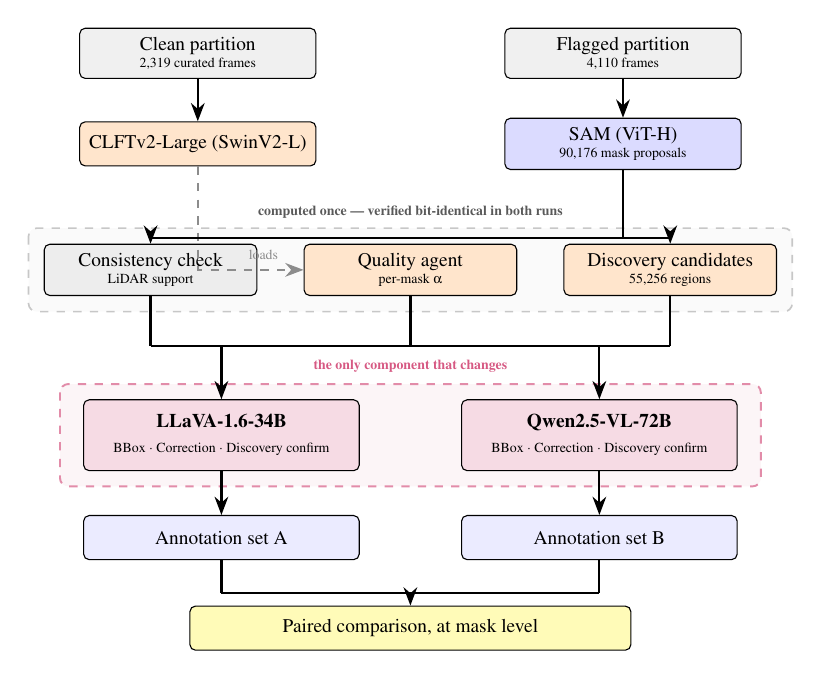
\begin{tikzpicture}[
  >=Stealth,
  every node/.style={font=\scriptsize},
  corpblock/.style={draw, rounded corners=2pt, align=center, fill=black!6,
                    minimum width=3.0cm, minimum height=0.56cm},
  samblock/.style ={draw, rounded corners=2pt, align=center, fill=blue!14,
                    minimum width=3.0cm, minimum height=0.56cm},
  swinblock/.style={draw, rounded corners=2pt, align=center, fill=orange!20,
                    minimum width=3.0cm, minimum height=0.56cm},
  detblock/.style ={draw, rounded corners=2pt, align=center, fill=gray!14,
                    minimum width=2.7cm, minimum height=0.56cm},
  vlmblock/.style ={draw, rounded corners=2pt, align=center, fill=purple!14,
                    minimum width=3.5cm, minimum height=0.90cm},
  annblock/.style ={draw, rounded corners=2pt, align=center, fill=blue!8,
                    minimum width=3.5cm, minimum height=0.56cm},
  cmpblock/.style ={draw, rounded corners=2pt, align=center, fill=yellow!28,
                    minimum width=5.6cm, minimum height=0.56cm},
  arr/.style={->, thick},
  lin/.style={thick},
  darr/.style={->, dashed, black!45, thick},
  stageLabel/.style={font=\tiny\bfseries, text=black!65},
]

%% ── Corpus ──────────────────────────────────────────────────────────────────
\node[corpblock] (clean) at (2.3, 0)
  {Clean partition\\[-2pt]{\tiny 2{,}319 curated frames}};
\node[corpblock] (flag) at (7.7, 0)
  {Flagged partition\\[-2pt]{\tiny 4{,}110 frames}};

\node[swinblock] (swinpre) at (2.3, -1.15)
  {CLFTv2-Large (SwinV2-L)};
\node[samblock] (sam) at (7.7, -1.15)
  {SAM (ViT-H)\\[-2pt]{\tiny 90{,}176 mask proposals}};

%% ── Shared, computed once ───────────────────────────────────────────────────
\node[detblock] (consist) at (1.7, -2.75)
  {Consistency check\\[-2pt]{\tiny LiDAR support}};
\node[detblock, fill=orange!20] (quality) at (5.0, -2.75)
  {Quality agent\\[-2pt]{\tiny per-mask $\alpha$}};
\node[detblock, fill=orange!20] (cand) at (8.3, -2.75)
  {Discovery candidates\\[-2pt]{\tiny 55{,}256 regions}};

%% ── The fork: the only thing that changes ───────────────────────────────────
\node[vlmblock] (runA) at (2.6, -4.85)
  {\textbf{LLaVA-1.6-34B}\\[1pt]{\tiny BBox $\cdot$ Correction $\cdot$ Discovery confirm}};
\node[vlmblock] (runB) at (7.4, -4.85)
  {\textbf{Qwen2.5-VL-72B}\\[1pt]{\tiny BBox $\cdot$ Correction $\cdot$ Discovery confirm}};

\node[annblock] (annA) at (2.6, -6.15) {Annotation set A};
\node[annblock] (annB) at (7.4, -6.15) {Annotation set B};

\node[cmpblock] (cmp) at (5.0, -7.30)
  {Paired comparison, at mask level};

%% ── Enclosures ──────────────────────────────────────────────────────────────
\begin{scope}[on background layer]
  \fill[gray!4, draw=black!22, dashed, rounded corners=3pt, line width=0.6pt]
    (0.15, -2.22) rectangle (9.85, -3.28);
  \fill[purple!4, draw=purple!45, dashed, rounded corners=3pt, line width=0.7pt]
    (0.55, -4.20) rectangle (9.45, -5.50);
\end{scope}

\node[stageLabel] at (5.0, -2.02) {computed once --- verified bit-identical in both runs};
\node[stageLabel, text=purple!65] at (5.0, -3.98) {the only component that changes};

%% ── Arrows ──────────────────────────────────────────────────────────────────
\draw[arr] (clean) -- (swinpre);
\draw[arr] (flag)  -- (sam);

\draw[darr] (swinpre.south) -- (2.3, -2.75)
  -- node[above, font=\tiny, pos=0.62]{loads} (quality.west);

%% SAM proposals fan out to the shared signals
\draw[lin] (sam.south) -- (7.7, -2.35);
\draw[lin] (1.7, -2.35) -- (8.3, -2.35);
\draw[arr] (1.7, -2.35) -- (consist.north);
\draw[arr] (8.3, -2.35) -- (cand.north);

%% shared signals feed both runs over one bus
\draw[lin] (consist.south) -- (1.7, -3.72);
\draw[lin] (quality.south) -- (5.0, -3.72);
\draw[lin] (cand.south)    -- (8.3, -3.72);
\draw[lin] (1.7, -3.72) -- (8.3, -3.72);
\draw[arr] (2.6, -3.72) -- (runA.north);
\draw[arr] (7.4, -3.72) -- (runB.north);

\draw[arr] (runA) -- (annA);
\draw[arr] (runB) -- (annB);

\draw[lin] (annA.south) -- (2.6, -6.85);
\draw[lin] (annB.south) -- (7.4, -6.85);
\draw[lin] (2.6, -6.85) -- (7.4, -6.85);
\draw[arr] (5.0, -6.85) -- (cmp.north);

\end{tikzpicture}
}
    \caption{
    The annotation system and the backend substitution setup.
    All signals above the fork are computed once and reused in both runs, including SAM proposals, the LiDAR consistency check, the segmentation‑quality scores, and the discovery candidates.
    Only the VLM block changes, so any differences between the two annotation sets come from the backend.
    Both runs use the same triage rule, applied under one revision, and only rejection removes pixels.
    }
    \label{fig:architecture}
\end{figure}


\section{\uppercase{Methodology}}
\label{sec:methodology}

Figure~\ref{fig:architecture} shows the system and the point at which the two runs diverge.
Everything above the fork is computed once and reused, so the VLM block is the only variable.

\subsection{Agents}

\subsubsection{Consistency agent}
A deterministic check measures the fraction of mask pixels containing projected LiDAR returns.  
Masks must exceed $\tau = 0.1$, which removes masks leaking into sky or void regions.  
This signal is identical across backends.

\subsubsection{Quality agent}
The Quality agent is a CLFTv2 cross‑fusion segmentation model with a SwinV2‑Large backbone, trained on the clean partition and referred to as Swin in the tables.
It takes the camera image together with the projected LiDAR depth map and predicts a dense class map at $384 \times 384$ once per frame; each mask is then compared to this map through agreement $\alpha$, the fraction of its pixels assigned to its annotated class.
Thresholds are class‑specific: $\tau_q^{\text{large}} = 0.30$ for vehicles and signs, and $\tau_q^{\text{small}} = 0.15$ for cyclists and pedestrians.  
Cyclists and pedestrians share one segmentation class, so $\alpha$ measures membership in the merged human class.  
The module is called an agent only because it produces a binary decision, reporting sufficient agreement when $\alpha \geq \tau_q$ and insufficient agreement otherwise.
Because it reads LiDAR as one of its two inputs, its verdict is not fully independent of the consistency check, a point the triage rule has to account for.

\subsubsection{BBox agent}
The BBox agent is the VLM-based classifier in the pipeline.  
It receives only a tight RGB crop and must choose exactly one word from a fixed vocabulary containing the four annotation classes (vehicle, sign, cyclist, pedestrian), the additional class traffic light, four background surfaces (vegetation, building, sky, snow), and three distractors (road, other, unclear).  
The annotated class is never mentioned in the prompt.  
An answer matching the annotation is treated as valid, with traffic light also valid for sign.  
Naming a background surface is treated as background and is strong evidence that the mask covers no object.  
Any other answer is read as a failure to recognise the annotated object, and a reply that cannot be read at all is treated as recognition.  
Because it performs a full VLM forward pass for every mask, the BBox agent is the main contributor to inference cost.

\subsubsection{Discovery agent}
The Discovery agent recovers objects SAM never proposed and is the only agent that adds pixels rather than removing them.  
It compares the segmentation map to the SAM annotation at $384 \times 384$ and extracts 8‑connected components where the model predicts an object class on pixels SAM leaves as background.  
Components smaller than 20 pixels are discarded and the largest 20 per frame are sent to the VLM, a cap that bounds cost per frame.
Candidate generation reads no VLM output at all, so both backends are offered the same set.
Each candidate is cropped from the full‑resolution image with padding, upscaled if needed, and passed as a single image.

Vehicle and sign candidates receive a presence‑confirmation question answerable with the class name or a word declining it.  
Human candidates receive a three‑way discrimination because the segmentation model merges cyclists and pedestrians while the annotation vocabulary separates them.  
This asymmetry matters because only human candidates require choosing between two classes rather than confirming one.

A candidate is confirmed only when the reply names an offered class, and unusable replies default to non‑confirmation.  
This failure convention is the opposite of the BBox agent’s: where an unparseable reply preserves a mask on the BBox path, it silently discards a candidate on this one.  
Failed candidates are retained and flagged so confirmation rates can be computed over answered candidates rather than over a denominator shrunk by serving faults.  
Confirmed components are upsampled and painted only onto pixels still marked as background, so discovery never overwrites existing labels and inherits the $384 \times 384$ quantisation of the segmentation map.

All discovery replies are stored in raw form and re‑parsed with a single parser, so confirmation rates are computed only over candidates the model actually answered.


\subsection{Triage rules}
\label{sec:triage}

\subsubsection{Accept}
A mask is accepted when all three agents agree that it is correct.  
The BBox agent recognises the annotated object, the Quality agent finds sufficient class agreement, and the consistency check passes.  
When all signals concur, the mask is written unchanged.

\subsubsection{Reject}
A mask is rejected when two of the three agents judge that it is wrong.  
The BBox agent may say the crop does not contain the annotated object, the Quality agent may say the segmentation does not match the class, and the consistency check may say the mask has insufficient LiDAR support.  
Any two of these disagreements remove the mask.

Two cases count as two disagreements immediately.
If the BBox agent names a background surface, that is direct evidence that the mask covers no object rather than absence of confirmation, so it removes the mask on its own.
A failure to recognise the object counts twice when the consistency check passes and the Quality agent also withholds support, and counts once when the Quality agent does support the mask, which protects small or ambiguous objects the VLM may misread on a tight crop.

Masks with degenerate geometry (extreme aspect ratio or too few pixels for the class) are rejected before any agent is called.

Thin or distant objects can trigger both the Quality agent and the consistency check for the same physical reason, since both read LiDAR.  
Lower thresholds for cyclists and pedestrians reduce this effect but do not remove it.  
Differences between backends arise mainly from cases where the BBox agent disagrees, because it is the only agent whose judgement changes with the backend.

\subsubsection{Retained, flagged}
A mask is retained when the agents do not agree strongly enough to delete it.  
This covers all cases with only one agent in disagreement.  
The mask is written unchanged, and the disagreement is marked for attention rather than used to remove pixels.  
For example, a mask that both the BBox agent and the Quality agent support but fails the consistency check has only one dissenting signal and is therefore retained.

\subsection{Dataset}
\label{sec:dataset}

This work builds on our earlier SAM-based annotation pipeline \cite{tahves2026samenhancedsegmentationroaddatasets}, which produced masks for all ZOD \cite{alibeigi2023zod} frames and split them into clean and flagged partitions.  
We revisit those annotations here: the flagged partition is re‑annotated under the multi‑agent system to evaluate and correct the SAM labels and to measure how VLM backend substitution changes those corrections.

The previous pass produced 2,319 clean frames and 4,135 flagged frames (Table~\ref{tab:dataset}).  
Twenty‑five flagged frames could not be annotated cleanly and are removed, leaving 4,110 frames and 90,176 mask proposals.

The flagged partition contains denser and more difficult scenes: 21.9 masks per frame versus 15.5 in the clean partition, and object pixels covering 3.64\% of the image versus 2.18\% (Table~\ref{tab:dataset_distributions}).  
Because our comparison is intentionally run on this harder half of the dataset, the verdict rates reported here should not be interpreted as typical for everyday driving scenes.

Two composition effects matter for reading the results.  
Signs make up half of all flagged masks, so backend behaviour on signs dominates any class‑pooled rate.  
Cyclists and pedestrians are rare: they cover only 0.31\% of flagged‑partition pixels, falling to 0.12–0.14\% at night and in snow.  
The classes where the two backends diverge most are therefore the ones with the least pixel evidence.

\begin{table}[h]
\centering
\caption{Dataset composition.}
\label{tab:dataset}
\begin{tabular}{lrrr}
\toprule
 & \textbf{Clean} & \textbf{Flagged} & \textbf{Total} \\
\midrule
Frames           & 2{,}319  & 4{,}135  & 6{,}454   \\
Vehicle masks    & 9{,}923  & 25{,}626 & 35{,}549  \\
Sign masks       & 19{,}056 & 46{,}066 & 65{,}122  \\
Cyclist masks    & 3{,}216  & 8{,}288  & 11{,}504  \\
Pedestrian masks & 3{,}864  & 10{,}781 & 14{,}645  \\
Total masks      & 36{,}059 & 90{,}761 & 126{,}820 \\
Masks per frame  & 15.5     & 21.9     & 19.7      \\
\bottomrule
\end{tabular}
\end{table}

\begin{table}[t]
\centering
\caption{Pixel-level class distribution by weather in the flagged partition.}
\label{tab:dataset_distributions}
\resizebox{\columnwidth}{!}{%
\begin{tabular}{lrcccc}
\toprule
\textbf{Weather} & \textbf{Frames} & \textbf{Veh.\,\%} & \textbf{Sign\,\%} & \textbf{Human\,\%} & \textbf{Object\,\%} \\
\midrule
Day -- fair   & 2{,}778 & 2.93 & 0.66 & 0.38 & 3.97 \\
Day -- rain   &    487 & 2.95 & 0.74 & 0.28 & 3.96 \\
Night -- fair &    612 & 1.42 & 0.66 & 0.14 & 2.22 \\
Night -- rain &    131 & 1.70 & 0.45 & 0.12 & 2.27 \\
Snow          &    127 & 2.49 & 0.71 & 0.13 & 3.33 \\
\midrule
All  & 4{,}135 & 2.66 & 0.66 & 0.31 & 3.64 \\
\bottomrule
\end{tabular}}
\end{table}


\subsection{Evaluation}
\label{sec:evaluation}

We compare two open‑weight VLM backends, LLaVA‑1.6‑34B \cite{liu2024llava} and Qwen2.5‑VL‑72B \cite{bai2025qwen25vl}, served on identical hardware on the TalTech HPC cluster using an NVIDIA A100\,80GB GPU.

\paragraph{Serving and decoding}
Both backends are served locally through Ollama, one model resident at a time, as the released tags \texttt{llava:34b} and \texttt{qwen2.5vl:72b}.
Each call sends the prompt and its images inline to the chat endpoint and asks for a complete response rather than a stream.
Decoding is greedy: temperature is zero, the context window is 2{,}048 tokens, and generation is capped at ten tokens, which is ample for a one‑word verdict.
Greedy decoding matters for the comparison, because it makes a run repeatable, so every difference reported below is a difference between models rather than between samples of one.
Four frames are processed concurrently.

\paragraph{Identical inputs}
Both models annotate the same 4,110 frames and 90,176 masks.
Each run sees the same mask identifiers, segmentation agreement values, LiDAR support, and discovery candidates.
Triage is recomputed offline under one rule, so differences arise only from the VLMs.
Prompts are identical and no per‑model tuning is applied.
The question is how far a fixed prompt set carries, not how well either model could be made to perform.

\paragraph{Verdicts reported as recorded}
A reply that cannot be read is replaced by a fallback verdict, so a recorded verdict is not always a judgement.
We report the rates the pipeline acted on, \emph{as recorded}, because those are the rates that produced the labels, and give the \emph{answered-only} rate beside them wherever the substitutions can be identified.
This is possible for Qwen; LLaVA's run predates the per-agent parse telemetry, so its substitutions cannot be separated from confident answers.
Since the BBox fallback counts as recognition, an as-recorded rate can only overstate the answered one, which fixes the direction of a difference even when one side cannot be decomposed.


\section{\uppercase{Results}}
\label{sec:results}

\subsection{Agent behaviour}

Figure~\ref{fig:qualitative} illustrates the five decision paths produced by the system.  
These examples show how the three agents interact: hallucinated masks are rejected when both judges concur, geometric failures remove pixels only when supported by a second signal, single-agent disagreements retain the mask, and discovery recovers objects missed by SAM.  
These behaviours are identical across backends; the differences reported below arise from the VLM verdicts that feed into these paths.

\begin{figure*}[t]
    \centering
    \begin{subfigure}[b]{0.19\textwidth}
        
\includegraphics[width=\linewidth]{figures/qual_halluc_a.png}\par\vspace{2pt}
        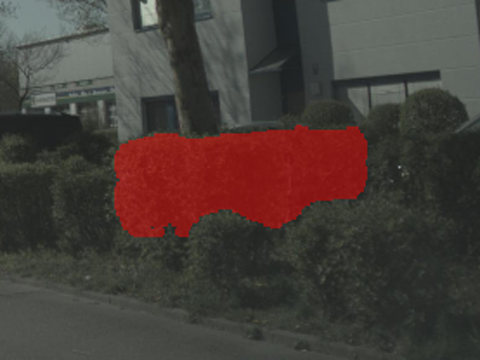
\includegraphics[width=\linewidth]{figures/qual_halluc_b.png}
        \caption{Hallucination}
    \end{subfigure}\hfill
    \begin{subfigure}[b]{0.19\textwidth}
        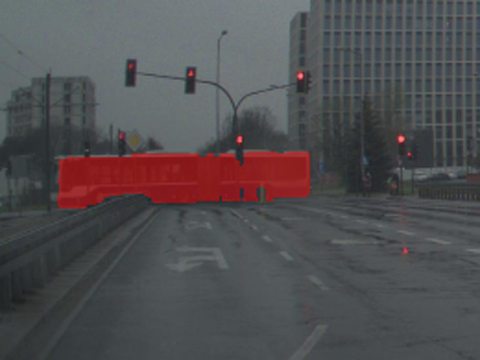
\includegraphics[width=\linewidth]{figures/qual_consistency.png}\par\vspace{2pt}
        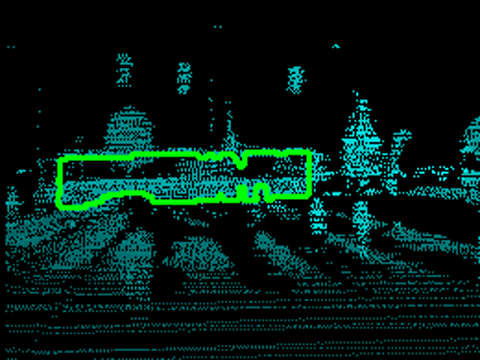
\includegraphics[width=\linewidth]{figures/qual_consistency_lidar.png}
        \caption{LiDAR fail, kept}
    \end{subfigure}\hfill
    \begin{subfigure}[b]{0.19\textwidth}
        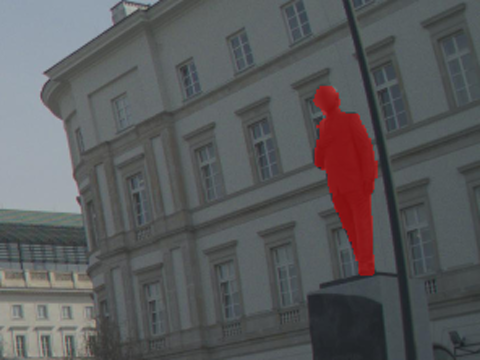
\includegraphics[width=\linewidth]{figures/qual_depthfail.png}\par\vspace{2pt}
        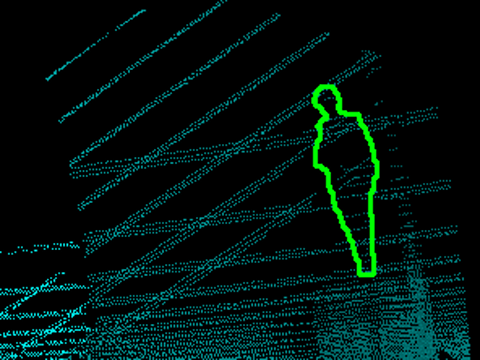
\includegraphics[width=\linewidth]{figures/qual_depthfail_lidar.png}
        \caption{LiDAR fail, deleted}
    \end{subfigure}\hfill
    \begin{subfigure}[b]{0.19\textwidth}
        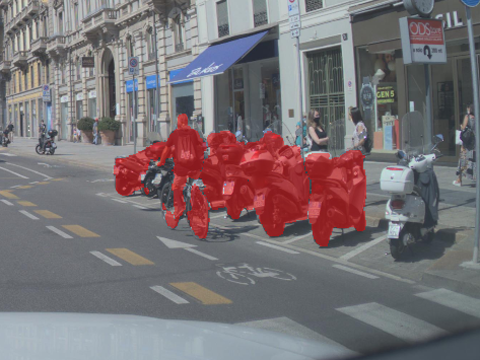
\includegraphics[width=\linewidth]{figures/qual_retain_downgrade.png}\par\vspace{2pt}
        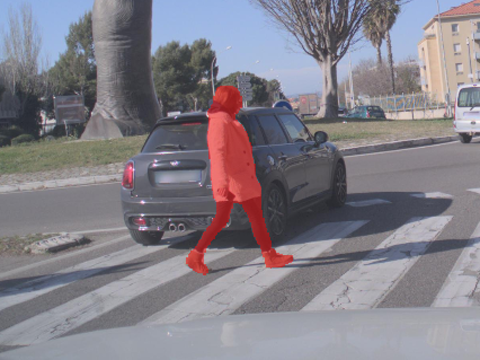
\includegraphics[width=\linewidth]{figures/qual_retain_quality.png}
        \caption{Disagreement}
    \end{subfigure}\hfill
    \begin{subfigure}[b]{0.19\textwidth}
        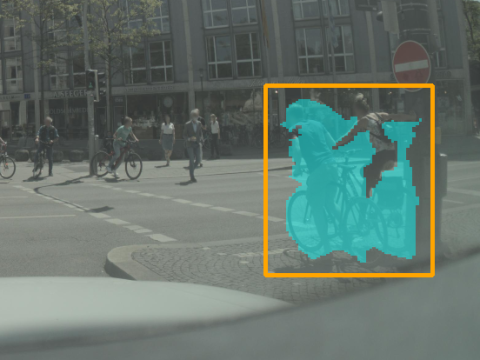
\includegraphics[width=\linewidth]{figures/qual_discovery_cyclist.png}\par\vspace{2pt}
        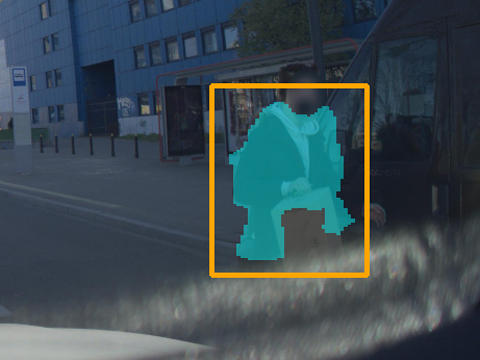
\includegraphics[width=\linewidth]{figures/qual_discovery_pedestrian.png}
        \caption{Discovery}
    \end{subfigure}
    \caption{The five decision paths of the multi-agent system, LLaVA-1.6-34B. Red overlay in (a)--(d) is the SAM mask under review; (b) and (c), lower panels, show LiDAR returns with the mask outlined in green. Cyan overlay in (e) is the Quality Agent's per-pixel prediction that seeds the discovery candidate; the orange box marks the region confirmed by the VLM.}
    \label{fig:qualitative}
\end{figure*}

% Generated by compare_models.py — do not edit by hand.
% Paired frame set: 4110 frames / 90176 masks.
% llava_34b: 4110 frames on disk; qwen2.5vl_72b_v2: 4110 frames on disk.
\begin{table}[t]
\centering
\caption{VLM agent behaviour on the 4{,}110 flagged frames both models completed (90{,}176 SAM masks, identical for both; Swin agreement and LiDAR consistency are VLM-independent and verified bit-identical across the two runs). Triage outcomes are the three reported outcomes of Section~\ref{sec:triage}, recomputed offline under the current deterministic rule for both models; \emph{retained, flagged} pools refinement and human review, which write identical labels. BBox rates are \emph{as-recorded}: they include masks whose verdict is a \textsc{safe\_default} substitution after an unparseable reply, which is what the pipeline acted on. Discovery outcomes are re-derived from the raw responses stored by both runs with a single parser, separating a model declining a candidate (\texttt{other}) from a reply the parser could not read at all; the hit rate is over answered candidates only. ``Human objects added'' counts confirmed cyclist and pedestrian candidates.}
\label{tab:agent_behavior}
\resizebox{\columnwidth}{!}{%
\begin{tabular}{lcc}
\toprule
\textbf{Metric} & \textbf{LLaVA-1.6-34B} & \textbf{Qwen2.5-VL-72B} \\
\midrule
\multicolumn{3}{l}{\textit{Triage outcomes (current rule, recomputed)}} \\
Accept & 43.2\% & 47.3\% \\
Reject & 20.9\% & 17.3\% \\
Retained, flagged & 35.8\% & 35.4\% \\
\addlinespace
\multicolumn{3}{l}{\textit{BBox VLM verdicts (as-recorded)}} \\
Valid (object present) & 62.1\% & 70.9\% \\
Invalid (object absent) & 35.6\% & 24.4\% \\
Background & \phantom{0}1.3\% & \phantom{0}3.6\% \\
\addlinespace
\multicolumn{3}{l}{\textit{Verdict provenance}} \\
\textsc{safe\_default} share of BBox & n/a\textsuperscript{a} & 11.3\% \\
Valid, answered only & n/a\textsuperscript{a} & 67.2\% \\
\addlinespace
\multicolumn{3}{l}{\textit{Per-class rejection rate}} \\
Vehicle & \phantom{0}5.1\% & 16.3\% \\
Sign & 26.0\% & 10.8\% \\
Cyclist & 46.5\% & 33.3\% \\
Pedestrian & 16.9\% & 35.4\% \\
\addlinespace
\multicolumn{3}{l}{\textit{Discovery (55{,}256 Swin-proposed candidates)}} \\
Confirmed & 45{,}578 & 45{,}538 \\
Declined (\texttt{other}) & 8{,}721 & 9{,}718 \\
Unparseable reply & 957 & 0 \\
Hit rate (answered only) & 83.9\% & 82.4\% \\
Human objects added & 6{,}376 & 3{,}506 \\
\addlinespace
\multicolumn{3}{l}{\textit{Discovery confirmation by prompt (answered only)}} \\
Vehicle & 83.0\% & 87.6\% \\
Sign & 84.2\% & 89.3\% \\
Human (cyclist/pedestrian) & 85.9\% & 45.3\% \\
\bottomrule
\end{tabular}}
\\[2pt]
\footnotesize\textsuperscript{a} The LLaVA run predates the per-agent parse telemetry in \texttt{vlm/health.py} and stored only the parsed verdict, so its \textsc{safe\_default} share is not recoverable offline. Its \emph{discovery} non-answer rate is measurable and is reported above.
\end{table}


\subsection{Backend divergence in mask judgement}

Table~\ref{tab:agent_behavior} gives the paired comparison for the BBox agent.  
Under identical prompts and identical non-VLM inputs, the two backends agree on only 57.0\% of mask-level judgements.  
Qwen is more permissive overall, returning \texttt{valid} on 70.9\% of crops versus LLaVA’s 62.1\% as recorded; its answered-only rate is 67.2\%.

The differences are strongly class-dependent.  
Qwen rejects fewer signs (10.8\% vs.\ 26.0\%) and cyclists (33.3\% vs.\ 46.5\%), but more vehicles (16.3\% vs.\ 5.1\%) and pedestrians (35.4\% vs.\ 16.9\%).  
A single acceptance rate hides this redistribution.

These shifts propagate into the labels.  
Recomputed under one triage rule, 40.3\% of masks receive different outcomes under the two backends.  
Of these, 16{,}985 masks (18.8\% of the corpus, 7.5 million pixels) are retained by one backend and rejected by the other.
Since only rejection removes pixels, backend choice determines which objects survive triage.
Figure~\ref{fig:flips} shows four of these masks, one per class, with every non-VLM input held identical.

\begin{figure*}[t]
    \centering
    \begin{subfigure}[t]{0.235\textwidth}
        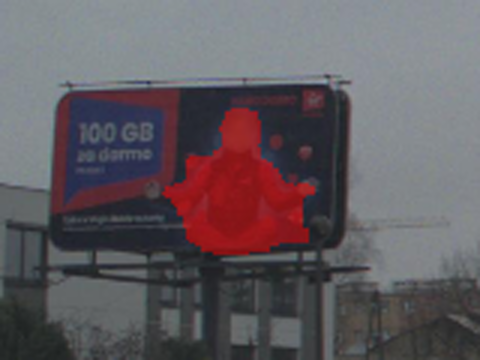
\includegraphics[width=\linewidth]{figures/qual_flip_pedestrian.png}
        \caption{Billboard: Qwen deletes}
    \end{subfigure}\hfill
    \begin{subfigure}[t]{0.235\textwidth}
        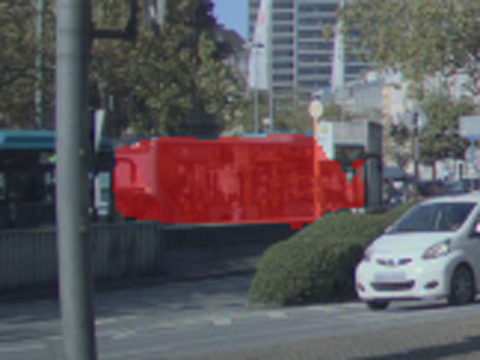
\includegraphics[width=\linewidth]{figures/qual_flip_vehicle.png}
        \caption{Bus: Qwen deletes}
    \end{subfigure}\hspace{5mm}
    \begin{subfigure}[t]{0.235\textwidth}
        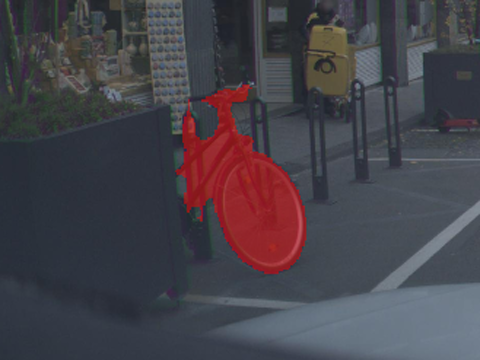
\includegraphics[width=\linewidth]{figures/qual_flip_cyclist.png}
        \caption{Cyclist: LLaVA deletes}
    \end{subfigure}\hfill
    \begin{subfigure}[t]{0.235\textwidth}
        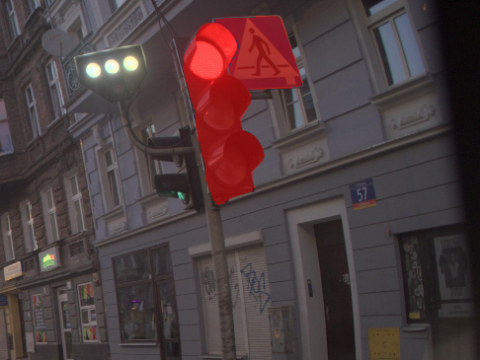
\includegraphics[width=\linewidth]{figures/qual_flip_sign.png}
        \caption{Sign: LLaVA deletes}
    \end{subfigure}
    \caption{Four of the 16{,}985 masks that one backend keeps and the other deletes, with the deleting backend named under each panel. Every input is shared: the same SAM mask, the same Swin agreement $\alpha$, and the same LiDAR support, all verified bit-identical across the runs (Section~\ref{sec:evaluation}), so the BBox verdict is the only difference.}
    \label{fig:flips}
\end{figure*}

% Generated by compare_models.py — do not edit by hand.
\begin{table}[t]
\centering
\caption{Agent signal agreement on the 90{,}176 paired masks from 4{,}110 frames both models completed. Reference positive $=$ Swin quality \textit{good} ($\alpha \geq \tau_q$, per-class threshold); masks without a Swin score (geometry-prefiltered) are excluded. Swin is a noisy judge rather than ground truth, but it is identical for both runs, so it ranks the two VLMs on one fixed yardstick. For Qwen the \emph{answered only} row excludes masks whose verdict is a \textsc{safe\_default} substitution; the equivalent row cannot be computed for LLaVA, whose run predates the parse telemetry. Cross-VLM BBox agreement: 57.0\% of masks receive the same verdict from both models.}
\label{tab:agent_performance}
\resizebox{\columnwidth}{!}{%
\begin{tabular}{lcccc}
\toprule
\textbf{Agent} & \textbf{Acc.} & \textbf{Prec.} & \textbf{Rec.} & \textbf{F1} \\
\midrule
BBox VLM (LLaVA-1.6-34B) & 64.1 & 72.0 & 71.1 & 71.5 \\
BBox VLM (Qwen2.5-VL-72B) & 63.7 & 69.0 & 77.8 & 73.1 \\
\quad Qwen, answered only & 67.5 & 75.6 & 76.4 & 76.0 \\
\bottomrule
\end{tabular}}
\end{table}


Table~\ref{tab:agent_performance} compares each backend to the Quality Agent.
That agent is not a ground truth, so the table does not measure correctness; it measures how far each backend's decision boundary sits from one fixed automated reference, and a backend could differ from it by being right.
On that yardstick LLaVA is the more balanced judge (precision 72.0, recall 71.1, F1 71.5), while Qwen trades precision for recall (69.0, 77.8, F1 73.1).
Restricting Qwen to answered masks raises its precision to 75.6 and accuracy to 67.5, which locates part of its apparent permissiveness in substituted verdicts rather than in the model.

\subsection{Backend divergence in discovery}

Given the same 55{,}256 candidates (Table~\ref{tab:agent_behavior}), the two backends confirm at nearly the same overall rate over answered candidates: 82.4\% for Qwen against 83.9\% for LLaVA.
On the two presence-confirmation prompts Qwen is in fact the more permissive of the pair, confirming 87.6\% of vehicle candidates against LLaVA's 83.0\% and 89.3\% of sign candidates against 84.2\%.
A study reporting one confirmation rate per model would conclude that the two backends behave alike.

The divergence appears on the human prompt.
When the candidate must be classified as cyclist or pedestrian, Qwen confirms 45.3\% of candidates, compared to LLaVA’s 85.9\%.  
This produces 3{,}506 human objects under Qwen and 6{,}376 under LLaVA from identical candidate regions.  
The 41-point gap is concentrated on the two classes the pipeline can least afford to lose.
The collapse is not the backend being generally more cautious, because the same backend is the more permissive of the two on the other two prompts.
What changes is the task the prompt encodes: confirming a presence transfers, choosing between two classes does not.

Taken together, the two VLM agents fail in different ways under the same prompt set.  
The BBox agent shifts its decision boundary differently for each class, and the discovery agent transfers on two prompts but collapses on the third.  
Portability must therefore be validated per agent and per class.

\subsection{Value of the discovery agent}
\label{sec:human}

% Generated from analyze_human_verification.py --only discovery, plus a paired
% frame bootstrap on the precision lift (5,000 resamples, seed 42).
% Labeled subset: 1,001 of 4,110 frames (24.4%); 13,695 of 55,252 candidates.
\begin{table}[t]
\centering
\caption{What the VLM confirmation gate buys on discovery candidates, against a human reference. \emph{Standalone} candidates cover regions where SAM segmented no object, so confirming one recovers a missed object; \emph{fringe} candidates are rims on objects SAM had already segmented, and are 70.3 percent of the population. \emph{Ungated} is the share of all candidates of that kind the labeler judged a real object, which is what painting every candidate would yield. \emph{Gated} is the same share among the candidates a backend confirmed, and \emph{lift} is the difference, with a 95 percent interval resampling frames. Both backends are scored on the same candidates by the same labeler, so the lift is paired; the ungated rates themselves are provisional (Section~\ref{sec:human}).}
\label{tab:discovery_gate}
\resizebox{\columnwidth}{!}{%
\begin{tabular}{lcc}
\toprule
\textbf{Metric} & \textbf{Standalone} & \textbf{Fringe} \\
\midrule
Candidates labeled & 4{,}043 & 9{,}652 \\
Frames & 915 & 969 \\
Share of all candidates & 29.7\% & 70.3\% \\
\addlinespace
Ungated (paint everything) & 27.3\% & 35.0\% \\
\addlinespace
\multicolumn{3}{l}{\textit{LLaVA-1.6-34B}} \\
Candidates confirmed & 67.8\% & 88.0\% \\
Gated precision & 27.6\% & 34.6\% \\
Lift & $+0.24$ & $-0.48$ \\
\phantom{Lift} 95\% CI & [$-0.82$, $+1.29$] & [$-0.92$, $-0.08$] \\
\addlinespace
\multicolumn{3}{l}{\textit{Qwen2.5-VL-72B}} \\
Candidates confirmed & 73.7\% & 86.3\% \\
Gated precision & 28.8\% & 34.2\% \\
Lift & $+1.43$ & $-0.89$ \\
\phantom{Lift} 95\% CI & [$+0.52$, $+2.33$] & [$-1.33$, $-0.44$] \\
\bottomrule
\end{tabular}}
\end{table}


Because the candidate set is generated without the VLM, confirming every candidate is a control: it is what the pipeline does with no gate at all.
A human labeler judged 13{,}695 candidates over 1{,}001 of the 4{,}110 frames, marking each as a real object of the proposed class or not (Table~\ref{tab:discovery_gate}).
Standalone candidates cover regions where SAM segmented nothing; fringe candidates extend boundaries on objects SAM already segmented, and are 70\% of the population.

On standalone candidates, 27.3\% of which are real objects before any confirmation, Qwen's gate raises precision by 1.43 points while discarding 26\% of candidates, and LLaVA's by 0.24 points, an interval spanning zero, while discarding 32\%.
On fringe candidates both gates are worse than no gate, by 0.48 points for LLaVA and 0.89 for Qwen, with both intervals excluding zero: the candidates they decline are more likely to be real than the ones they confirm.
Coverage is a quarter of the frames and a single labeler whose strictness is still tightening, so the base rates are provisional; the lift is paired across backends and is the finding, and it has only shrunk as the reference has tightened.

This is the agent where backend substitution has its largest effect (a 41-point swing that moves 2{,}870 human objects between annotation sets), and also the agent whose verdict contributes least to precision.  
Backend substitution changes the labels; it does not guarantee improvement.

\subsection{Cost of the larger backend}

% Generated by compare_models.py — do not edit by hand.
\begin{table}[t]
\centering
\caption{
Inference cost on the 4{,}110 frames and 90{,}176 masks completed by both models. 
}

\label{tab:timing}
\resizebox{\columnwidth}{!}{%
\begin{tabular}{lcc}
\toprule
\textbf{Metric} & \textbf{LLaVA-1.6-34B} & \textbf{Qwen2.5-VL-72B} \\
\midrule
\multicolumn{3}{l}{\textit{Per-mask VLM latency (s)}} \\
BBox call, mean & \phantom{0}3.54 & 11.39 \\
BBox call, p90 & \phantom{0}4.97 & 15.99 \\
Swin quality (shared, per mask) & \phantom{0}$<$0.01 & \phantom{0}$<$0.01 \\
\addlinespace
\multicolumn{3}{l}{\textit{Per-frame wall time (s), median}} \\
Triage phase & 68.0 & 217.8 \\
Discovery phase & 40.8 & 132.0 \\
Total & 109.0 & 352.2 \\
\addlinespace
\multicolumn{3}{l}{\textit{Total time}} \\
Aggregate GPU-time & 132.3h & 426.9h \\
Wall-clock (4 workers) & \phantom{0}33.1h & 106.7h \\
\addlinespace
\multicolumn{3}{l}{\textit{VRAM (single A100-80GB)}} \\
Total & $\sim$22GB & $\sim$51GB \\
\bottomrule
\end{tabular}}
\end{table}


Table~\ref{tab:timing} reports runtime.  
The BBox agent dominates cost: 3.54 seconds per call for LLaVA and 11.39 seconds for Qwen.  
Annotating the 4{,}110 frames required 132.3 GPU-hours with LLaVA and 426.9 GPU-hours with Qwen, a factor of 3.2.  
VRAM usage is approximately 22 GB for LLaVA and 51 GB for Qwen.

Against this cost, Qwen is less selective, differs by 41 points on human discovery, and offers at most 1.4 points of precision on the candidates that matter.
The additional cost produces a different annotation distribution, not a better one on any metric measured here.

\subsection{Scope of these findings}

Two backends give one pairwise comparison, which cannot separate a property of VLM-judge pipelines from a property of these two models.
We therefore claim no generality for the constants: a third backend could place 57.0\% agreement, or a 41-point prompt collapse, at the centre of a distribution or at its edge, and nothing here distinguishes those.

Two findings survive that limitation, because they rest on contrasts within a backend rather than on the size of a gap between backends.
The first is the discovery collapse: the backend that loses 41 points on the human prompt is the more permissive of the two on the other two prompts, so the failure cannot be a global disposition and belongs to the task the prompt encodes.
The second is the class redistribution: the same backend rejects more vehicles and pedestrians while rejecting fewer signs and cyclists, so substitution moves the decision boundary differently per class rather than shifting selectivity uniformly.
A model that were simply stricter, or simply weaker, would produce neither pattern.
Neither statement needs a third backend.

What this study offers is therefore the protocol rather than the constants.
A substitution can be localised to an agent and to a class on identical inputs, the localisation is what a pooled acceptance rate destroys, and a pipeline that never measures it will not notice the point at which its labels change.


\section{Conclusion}

Our results show that replacing the VLM backend inside a fixed annotation system produces large and measurable shifts in behaviour.  
Under identical prompts and identical non‑VLM inputs, the two backends agree on only 57\% of crop‑level decisions.  
These differences are strongly class‑dependent: Qwen rejects 10.8\% of signs and 33.3\% of cyclists, while LLaVA rejects 26.0\% and 46.5\% respectively.  
The largest gap appears in discovery, where human candidate confirmations fall from 85.9\% under LLaVA to 45.3\% under Qwen.  
These shifts propagate directly into the final labels.  
Across the 4,110 frames, 18.8\% of masks, 7.5 million pixels, are kept by one backend and removed by the other.  
This shows that backend choice determines which objects survive triage, and that portability must be validated per agent and per class on identical inputs.




\section*{\uppercase{Acknowledgements}}

\begin{itemize}
  \item Conflicts of Interest: The authors declare no conflicts of interest or competing interests.
  \item Financial and Other Support: This work was funded by the European Union’s Horizon 2020 Programme under grant No.\ 856602 (Finest Twins) and Horizon Europe under grant No.\ 101135988 (PLIADES).
  \item Data Sharing: The agent implementations, verbatim prompts, and stored model responses used to compute every rate in this paper are available at \url{https://github.com/taltech-av/paper-vlm-annotation-pipeline}. Because responses are stored verbatim, all reported rates can be re‑derived offline without re‑running VLM inference.
  \item AI Tools: Claude Code (Anthropic) assisted with implementing the annotation pipeline, analysis scripts, and with drafting and editing the text. All experiments were designed and executed by the authors, and all results, figures, and claims were verified by the authors, who take full responsibility for the content.
\end{itemize}


\bibliographystyle{apalike}
{\small
\bibliography{references}}

\end{document}
